\section{Auswertung}
\label{sec:Auswertung}

\subsection{Anmerkungen zur Auswertung} % (fold)
\label{sub:anmerkungen_zur_auswertung}
	Der von den Autoren genutzte Versuchsaufbau produzierte in Verbindung mit dem Anweisungen, wie zu messen war, keine sinnvollen Daten. Deswegen stammen die Daten für die $\eta$-Messung von der parallel arbeitenden Gruppe\footnote{\emph{Sonja Terpoorten, Saskia Müller}}.


\subsection{Prismeninnenwinkel}
\label{sub:prismeninnenwinkel}
	Die Messergebnisse nach \ref{equ:phi} sind in der Tabelle~\ref{tab:innenw} zusammengefasst. Durchschnittlich ergibt sich ein Innenwinkel von \num{65.9+-1.9}~Grad, was den erwarteten 60~Grad eines gleichseitigen Dreiecks nahekommt.

	\begin{table}[H]
    \centering
    \caption{Messung des Prismeninnenwinkels.}
    \label{tab:innenw}
    \begin{adjustbox}{center}
    \begin{tabular}{
        S
        S}
     \toprule
     \multicolumn{1}{c}{$\phi_l$ in Grad} &
     \multicolumn{1}{c}{$\phi_r$ in Grad} \\
     \midrule
     \primitiveinput{../table/phi-messung.tex}
     \bottomrule
    \end{tabular}
    \end{adjustbox}
	\end{table}

	Im weiteren werden 60~Grad als Innenwinkel benutzt, da die restlichen Daten von einem anderen Prisma stammen (s.o.) und nicht sichergestellt werden kann, dass das Prisma immer mit der gleichen Seite in den Strahlengang gestellt wurde.


\subsection{Brechungsindices}
\label{sub:brechungsindices}
	Durch die Winkelmessung beim symmetrischen Strahlgang ergeben sich die Winkel aus Tabelle~\ref{tab:eta} für die einzelnen Spektrallinien der HgCd-Lampe. Daraus berechnen sich nach \ref{equ:brech} die nebenstehenden Brechungsindices.\\

	\begin{table}[H]
    \centering
    \caption[protection]{Spektrum der HgCd-Lampe. Die Wellenlängen der hellsten Emissionslinien von Quecksilber und Cadmium sind Literaturwerte\footnote{nach NIST, siehe Anhang.}, die anhand ihrer Farbe und Helligkeit zugeordnet worden sind.}
    \label{tab:eta}
    \begin{adjustbox}{center}
    \begin{tabular}{
        c
        c
        c
        c
        c
        c}
     \toprule
     \multicolumn{1}{c}{$\Omega_l$ in Grad} &
     \multicolumn{1}{c}{$\Omega_r$ in Grad} &
     \multicolumn{1}{c}{$\eta$ in rad} &
     \multicolumn{1}{c}{$n$} &
     \multicolumn{1}{c}{$\lambda$ in \si{\angstrom}} \\
     \midrule
     \primitiveinput{../table/brechungsin.tex}
     \bottomrule
    \end{tabular}
    \end{adjustbox}
	\end{table}


\subsection{Dispersionskurve}
\label{sub:dispersionskurve}
    \begin{figure}[H]
      \centering
      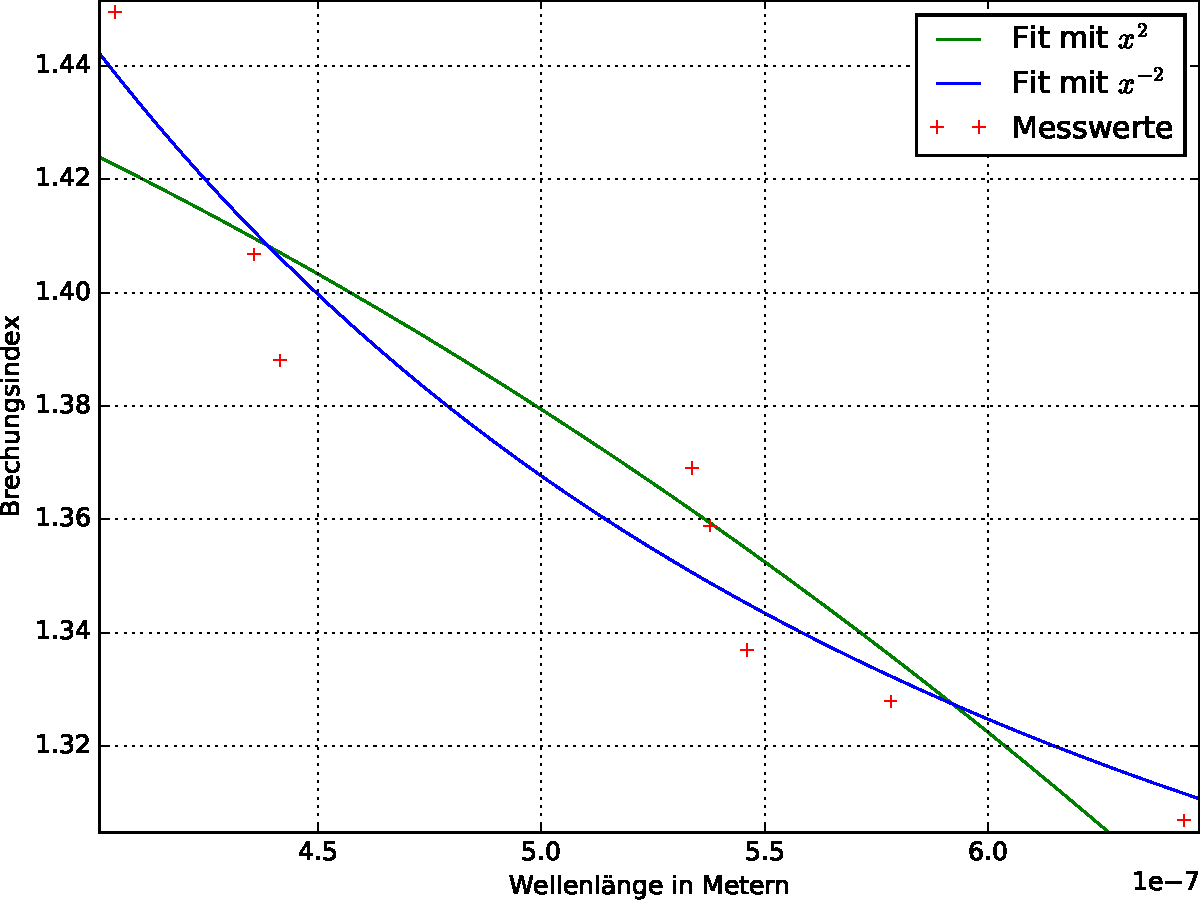
\includegraphics[width=0.6\textheight]{../plots/dispersionskurve.pdf}
      \caption{Abhängigkeit des Brechungsindexes von der Lichtfarbe.}
    \label{fig:dispersion}
    \end{figure}

    Das graphische Auftragen der Lichfarbe gegen die berechneten Brechungsindices ergibt Abbildung~\ref{fig:dispersion}. Es wurde zwei möglich Fits\footnote{Die Parameter wurden mithilfe des \emph{Simplex}-Algorithmus, die Fehler derselben mit dem \emph{Levenberg-Marquardt}-Algorithmus bestimmt.} eingezeichnet:
    \begin{align}\label{equ:fits}
        {n'}^2    =&  a'_0 + a'_2 x^2\\
        n^2     =&  a_0 + a'_2/x^2
    \end{align}
    Die Fitparameter lauten
    \begin{align}\label{equ:params}
        a'_0 =& \num{2.25+-0.06} \\
        a'_2 =& \SI{-1.40+-2.06}{10^{12} \m^2}\\
        a_0 =& \num{1.49+-0.04} \\
        a_2 =& \SI{-9.47+-1.05}{10^{-14} \m^2}.
    \end{align}

    Die Summe der Abweichungsquadrate ist
    \begin{align}\label{equ:abweichungsquad}
        s_{n'}^2  =& \num{2.86e-4}\\
        s_n^2   =& \num{1.68e-4} \;,
    \end{align}
    somit fittet die zweite, ungestrichene Gleichung besser. 
    Es ist auffällig, dass die Daten stark streuen.


    Numerisch findet sich eine Nullstelle von n und damit ein Absorptionsmaximum bei \SI{3.71e9}{\m}. Dieser Wert ist unrealistisch. Flintglas absorbiert im nahen Infrarot (\SI{>680}{\nano\m}) und im UV-Bereich (\SI{<300}{\nano\m})\footnote{Schott, siehe Anhang.}.


\subsection{Weitere Prismenparameter} 
\label{sub:weitere_prismenparameter}
    Die Abbesche Zahl\footnote{
    Verwendete Frauenhoferlinien:
    $\lambda_F = \SI{486}{\nano\m}$,
    $\lambda_D = \SI{589}{\nano\m}$,
    $\lambda_C = \SI{656}{\nano\m}$
    } ergibt sich mit 
    \begin{align}\label{equ:abbe}
        \frac{n(\lambda_D)-1}{n(\lambda_F)-n(\lambda_C)} = \num{4.87} \;.
    \end{align}
    Flintglas hat typischerweise eine Abbesche Zahl zwischen 20 und 55\footnote{Schott, siehe Anhang.}. Klassische Gläser können keine negative Abbesche Zahl besitzen. 

    Das Auflösungsvermögen des Prismas (es wird angenommen, dass das Prisma eine Kantenlänge von $b=\SI{3}{\centi\m}$ hat) berechent sich nach
    \begin{align}\label{equ:auloes}
        \frac{\lambda}{\Delta\lambda} = b \frac{\mathrm{d}n}{\mathrm{d}\lambda}\;.
    \end{align}
    Für die C-Frauenhoferlinie beträgt es
    \begin{align}
            A_C = \num{7661}
    \end{align}
    und für die F-Linie
    \begin{align}
        A_F = \num{17652} \;.
    \end{align}
    Diese Werte erscheinen zu hoch, das Spektroskop müsste zum Beispiel bei rotem Licht Wellenlängen separieren können, die sich um weniger als \SI{1}{\angstrom} unterscheiden. In der Praxis kann eine solche Auflösung schon allein wegen geringen Laufzeitschwankungen des Lichtstrahls mit endlicher Dicke (etwa durch Temperaturfluktuationen in der Luft) nicht erreicht werden. 